\section{Case Study}

%\subsection{Highway Corridor Capacity}

The state of California has large population concentrations in its northern and southern regions. These regions are connected by a highway corridor which runs through more sparsely populated agricultural areas in the San Joaquin Valley in the center of the state. Most road traffic between the states densely populated regions will follow a road corridor defined by Interstate 5 to the west and CA-99 to the east. This corridor is referred to as the 5-99 Corridor. The 5-99 corridor and all California cities with a population of greater than or equal to 50 thousand are shown in Figure \ref{fig:places_corridor}.

\begin{figure}[H]
	\centering
	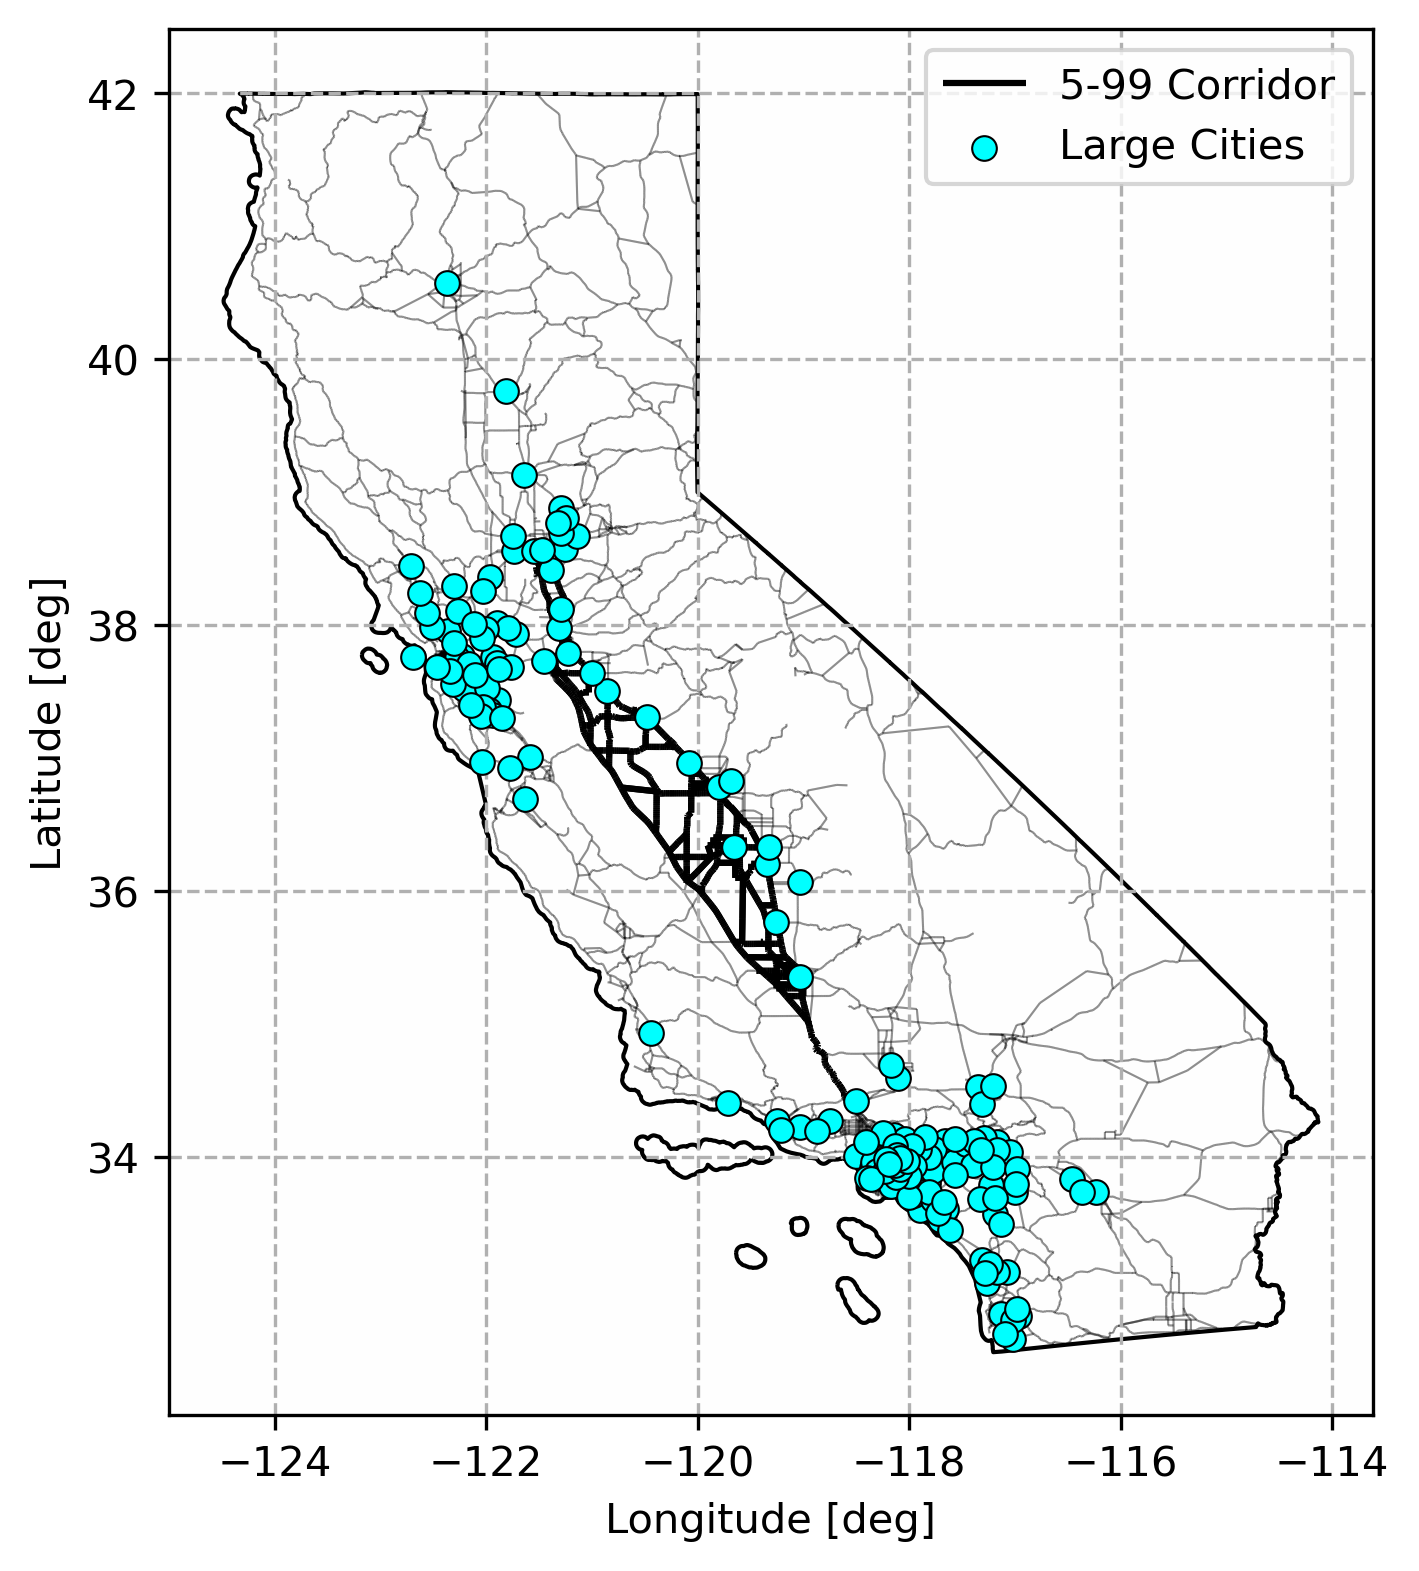
\includegraphics[width = \linewidth]{./figures/places_corridor.png}
	\caption{5-99 Corridor and California Cities with $\geq 50,000$ population.}
	\label{fig:places_corridor}
\end{figure}

The 5-99 corridor is of vital importance to road traffic in the state of California. Because of the large distance covered by the corridor, most \glspl{bev} will have to charge at a DC charging station in order to complete their itineraries in a reasonable amount of time. DC Charging stations can be divided into those which use the CCS plug and those which use the Tesla/NACS plug. At present, there are 344 CCS and 47 NACS stations in the 5-99 corridor per AFDC \citep{afdc_2023} with 1,029 and 901 chargers respectively. The locations and port counts for the CCS and NACS stations are shown in Figure \ref{fig:stations_corridor}.

\begin{figure}[H]
	\centering
	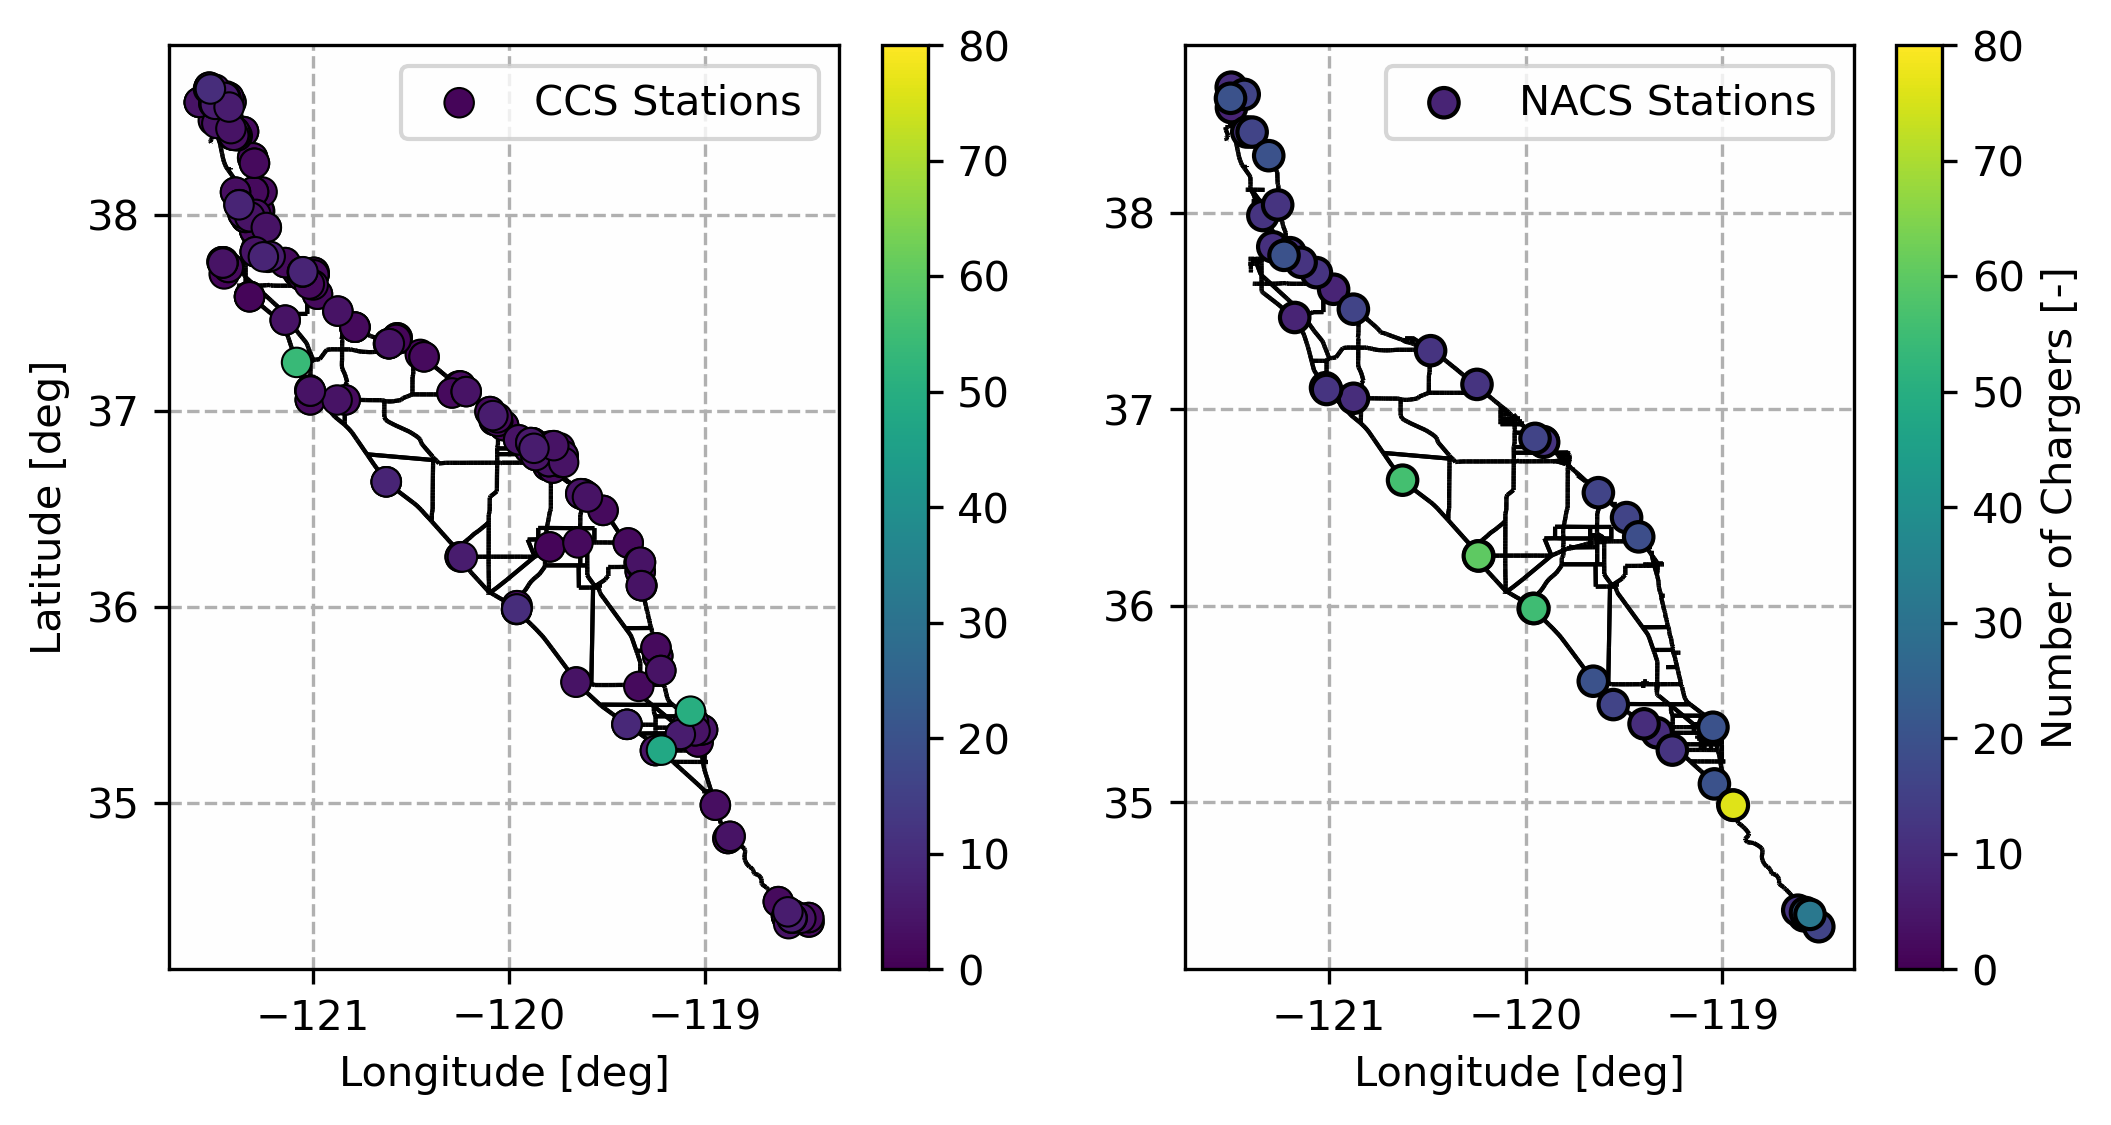
\includegraphics[width = \linewidth]{./figures/stations_corridor.png}
	\caption{Locations and sizes of DC charging stations up to 20 chargers in 5-99 Corridor.}
	\label{fig:stations_corridor}
\end{figure}

The NACS stations in the 5-99 corridor are, in general, larger and further apart than the CCS stations. Survival functions for station size by plug type are shown in Figure \ref{fig:stations_survival}.

\begin{figure}[H]
	\centering
	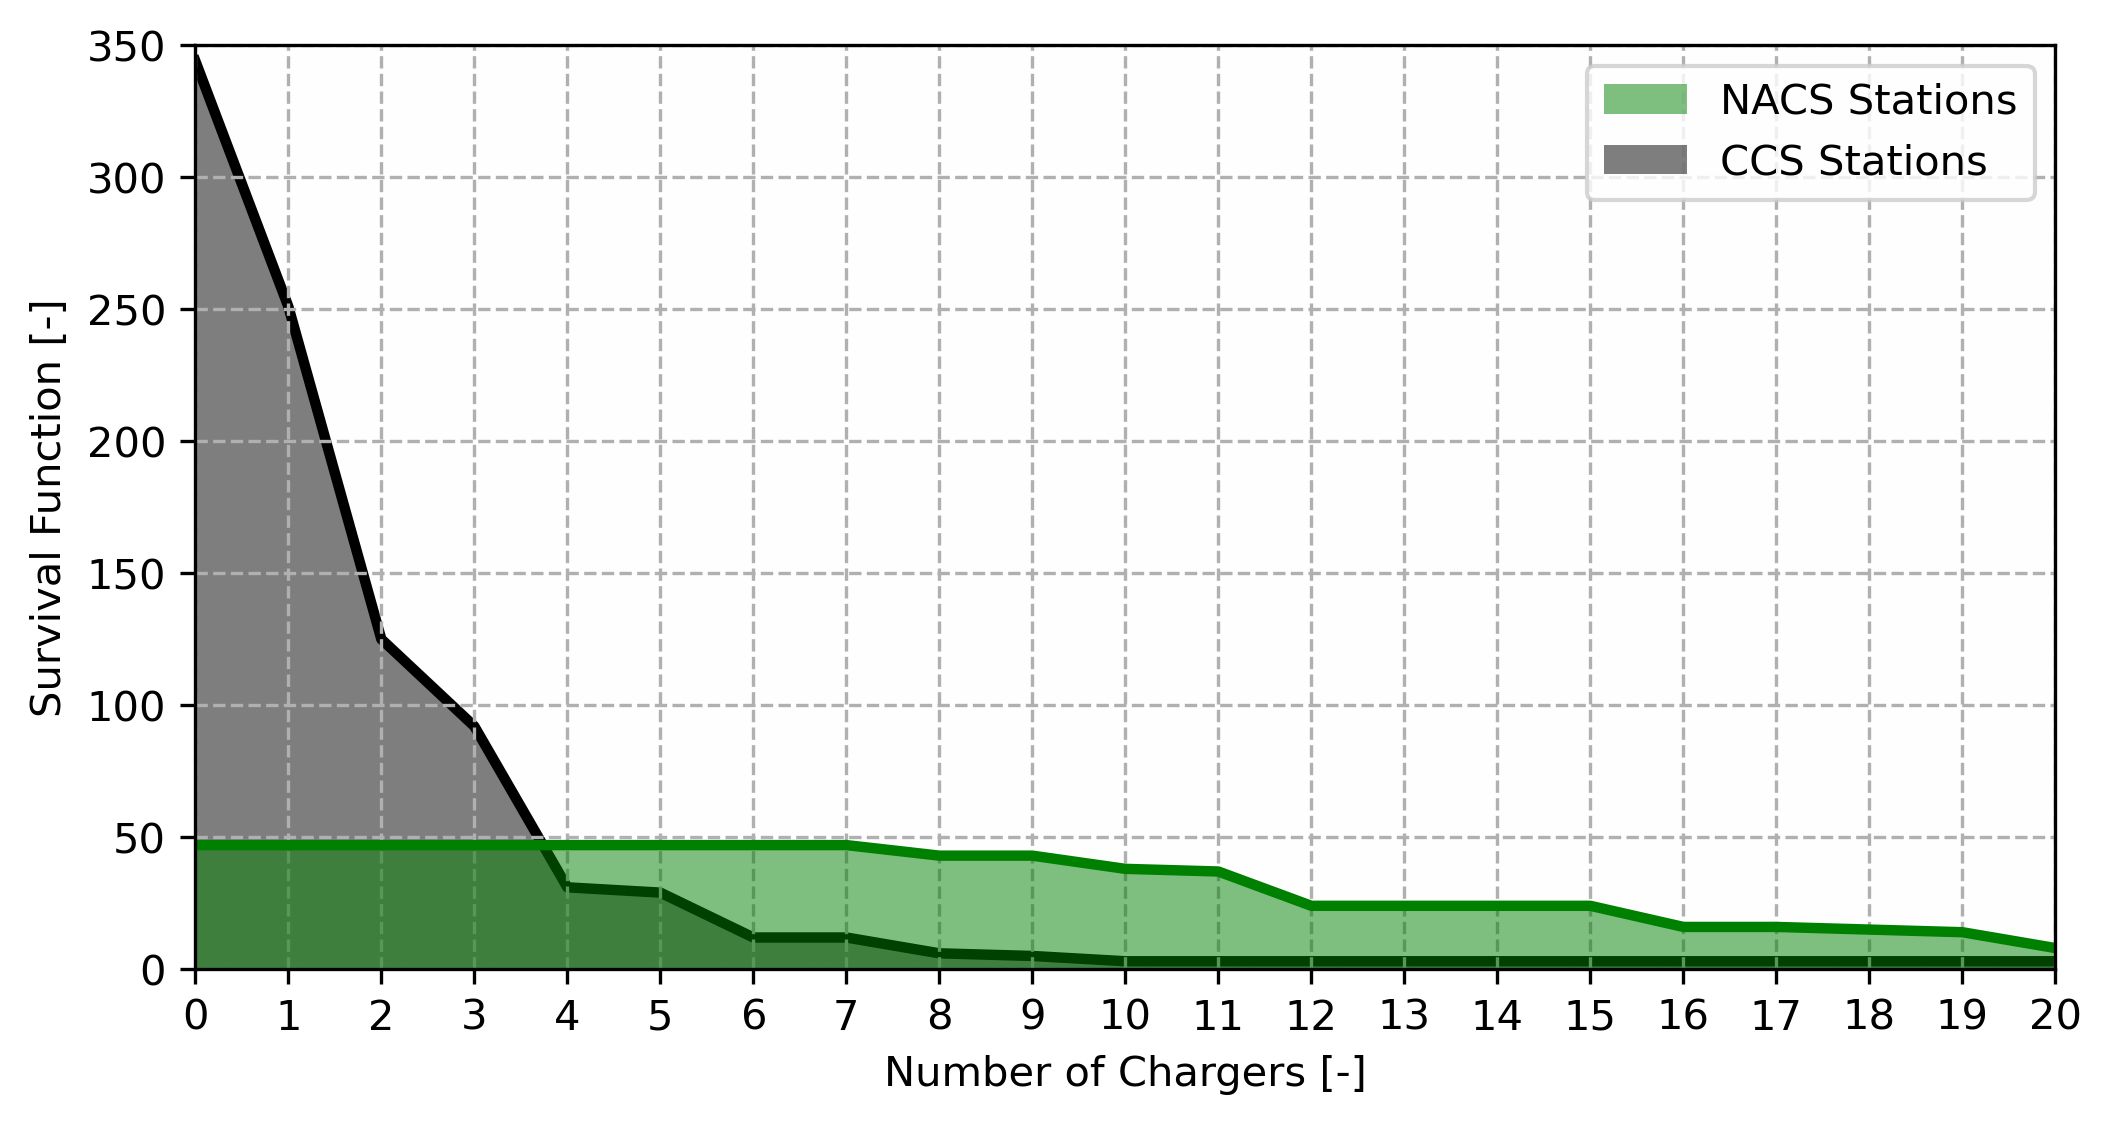
\includegraphics[width = \linewidth]{./figures/stations_survival.png}
	\caption{Survival functions for 5-99 corridor station size (port count) by plug type.}
	\label{fig:stations_survival}
\end{figure}

A second distance is charging speeds. Tesla chargers and vehicles are capable of charging at high rates, most commonly 150 kW or 250 kW. Non-Tesla chargers frequently have maximum charging rates in the range of 50 kW to 80 kW. In the 5-99 corridor, the vast majority of the Tesla chargers are of the 250 kW variety while 60\% of CCS chargers have maximum rates less than 150 kW and 80\% less than 250 kW. Vehicles which use the CCS infrastructure may also act as a charging speed bottleneck, often with maximum charging rates lower than that of the charger [SOURCE - EV Database].

A first question is how much travel can the current \gls{esn} accommodate. In order to answer this it is necessary to predict travel demand. Inter-city travel demand was generated using a travel gravity model [SOURCE]. Populations were taken from the US Census Bureau [SOURCE] and a friction function was fitted from NHTS Long Trip Survey data [SOURCE]. The distances used for the gravity model were based on the shortest-time-paths between cities. Where a shortest path did not go through the 5-99 corridor (between San Francisco and San Jose as an example), or the shortest path was short enough to not require charging (Sacramento to Stockton for example) the demand for that pair was not considered in the optimization. The vehicle range used was 300 km, a typical practical range for a modern \gls{bev} [SOURCE - EV Database]. The remaining demands were converted into fractions of overall demand such that they could scale with overall demand. Following this, for those origin-destination pairs remaining, a maximum acceptable travel time was computed by computing the time the shortest path would take if the vehicle could charge at any location at a low rate (3.3 kW). If congestion causes travel times exceed this level, then the DC \gls{esn} is no longer providing benefit.

Using demand fractions generated by the gravity model it is possible to compare the performance of an \gls{esn} subject to varying levels of demand. Some vehicles will be limited to using only one plug type while some may use either. The optimal performances of the CCS, NACS, and combined \glspl{esn} with increasing demand is displayed in Figure \ref{fig:esn_performance}.

\begin{figure}[H]
	\centering
	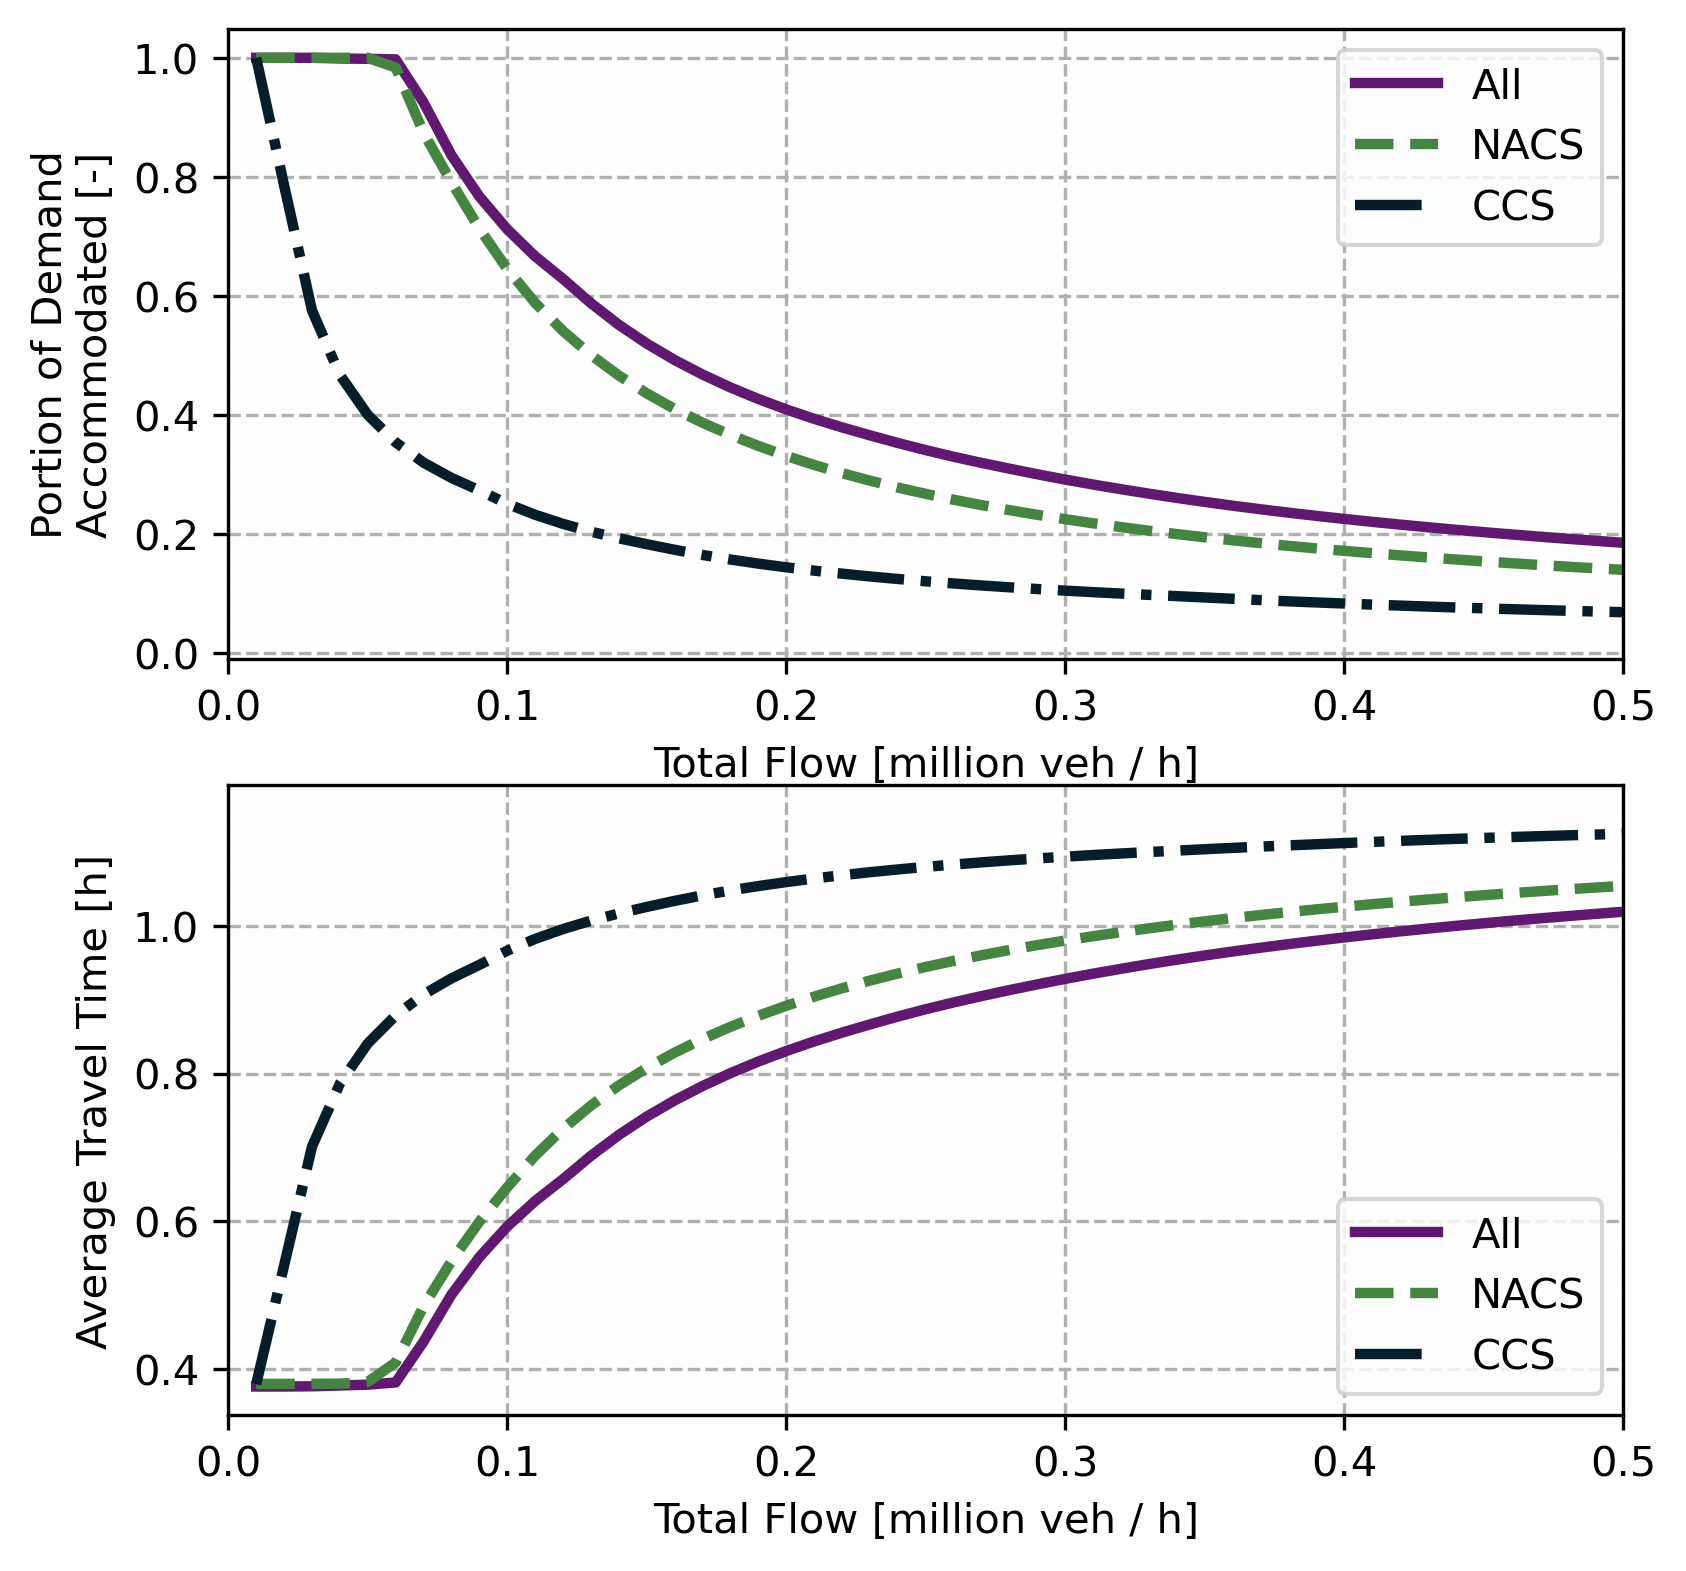
\includegraphics[width = \linewidth]{./figures/esn_performance.png}
	\caption{Performance of CCS, NACS, and combined \glspl{esn} with increasing demand.}
	\label{fig:esn_performance}
\end{figure}

The range of demand used in Figure \ref{fig:esn_performance} is reflective of the range of hourly vehicle flows seen on Interstate 5 in the San Joaquin Valley [SOURCE https://dot.ca.gov/programs/traffic-operations/census/traffic-volumes/2017/route-5-6]. At the end of 2023, \glspl{bev} accounted for around 4\% of the California light-duty vehicle fleet \citep{cec_2024} and, likely a similar portion of light-duty vehicle trips. At this volume, some congestion should be seen at CCS stations but very little should be seen at NACS stations and this appears to be the case [SOURCE - https://www.ucdavis.edu/blog/charging-not-range-becoming-top-concern-electric-car-drivers] although data is very hard to come by. The model presented, and what data can be found, suggest that the configuration of the NACS \gls{esn} is more efficient on a effective-capacity-per-charger basis. Some of the delta is based on the difference in charger speeds which favors the NACS \gls{esn}. The majority of the difference is due to the more centralized structure of the NACS network, being composed of more efficient stations. The differences in station size distribution between the CCS and NACS networks are stark. Both networks have a small number of very large stations clearly intended for high volume usage. The main difference is that the remainder of NACS stations are mid-sized, in the range of 10 to 25 chargers, while the remainder of CCS stations are small, in the range of 1 to 4 chargers.

The benefit of a more distributed network is that, by virtue of having more station locations, it is more likely to have a station closer to a demand node and to require fewer and shorter deviations out-of-path for travel demand. There are also more candidate locations which can accommodate a smaller station. The stations located in the 5-99 corridor serve local demand as well as thru-traffic, local demand may even be their primary purpose. As seen in \citep{Liu_2023}, larger stations are also favored for nodal demand if queuing is considered. However, drivers looking to charge their vehicles then return to their starting location can only go so far before the energy expended on the return leg renders the trip pointless. This means that more and better sited locations bring a real benefit. The preference for large stations is more pronounced for travel demand. Given modern \gls{bev} ranges and the concentration of long-distance traffic on limited access highways, long-distance travelers are less sensitive to the location advantages of smaller stations but benefit from the greater queue dissipation efficiency of larger stations.

A planner might be interested to know how the CCS network could be improved to perform more similarly to the NACS network given a limited budget. To answer this question, the CCS network was optimally expanded for budgets of 10, 25, 50, and 100 chargers to be assigned to existing stations. The locations and scales of additions are shown in Figure \ref{fig:augmented_esns}.

\begin{figure}[H]
	\centering
	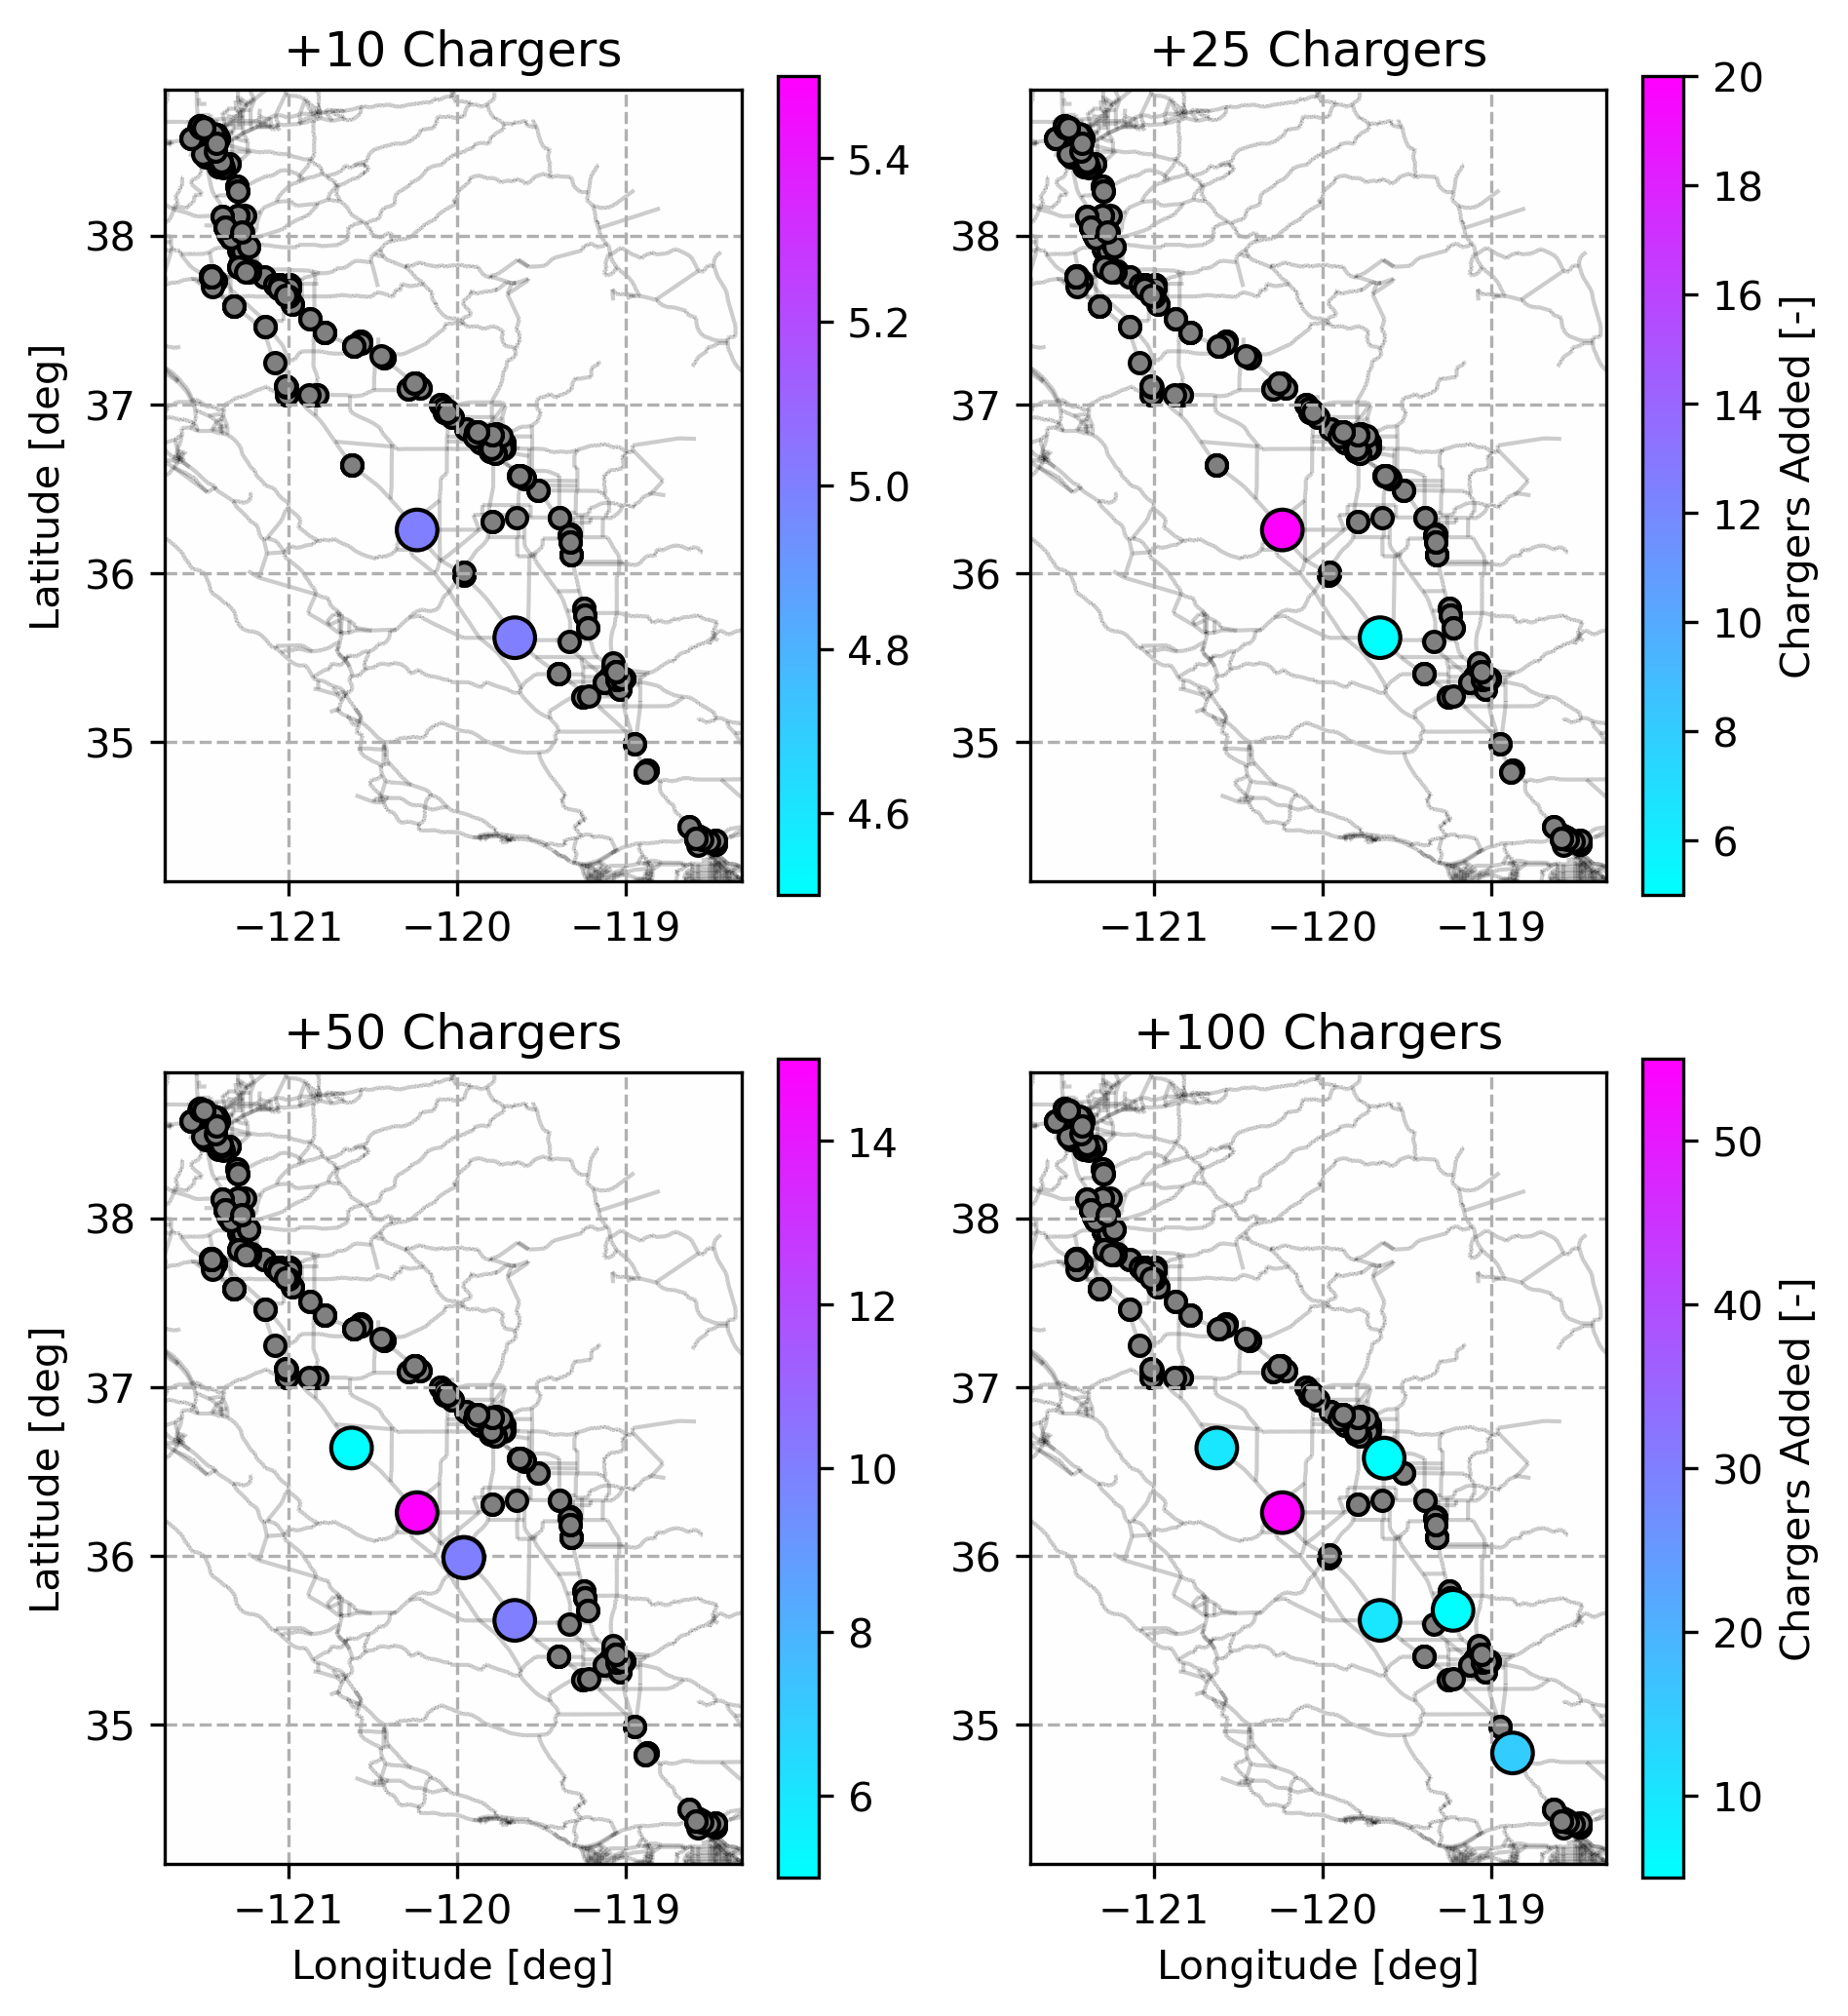
\includegraphics[width = \linewidth]{./figures/augmented_esns.png}
	\caption{Optimal allocations of 10, 25, 50, and 100 additional chargers for CCS \gls{esn}.}
	\label{fig:augmented_esns}
\end{figure}

The optimal allocations of additional chargers broadly favor large stations on Interstate 5 and towards the center of the corridor. This is an intuitive allocation. The 5-99 corridor is of a distance where vehicles from many, but not all, cities can reach the half-way point before needing to charge. Interstate 5 is on the shortest road-path for many more origin-destination pairs than CA-99 is. Adding large stations in this area should substantially improve the corridor for travelers moving from norther California to southern California. It is not a coincidence that large Tesla stations are located in the same area. The additional chargers impact on corridor performance is shown in Figure \ref{fig:augmented_esn_performance}.

\begin{figure}[H]
	\centering
	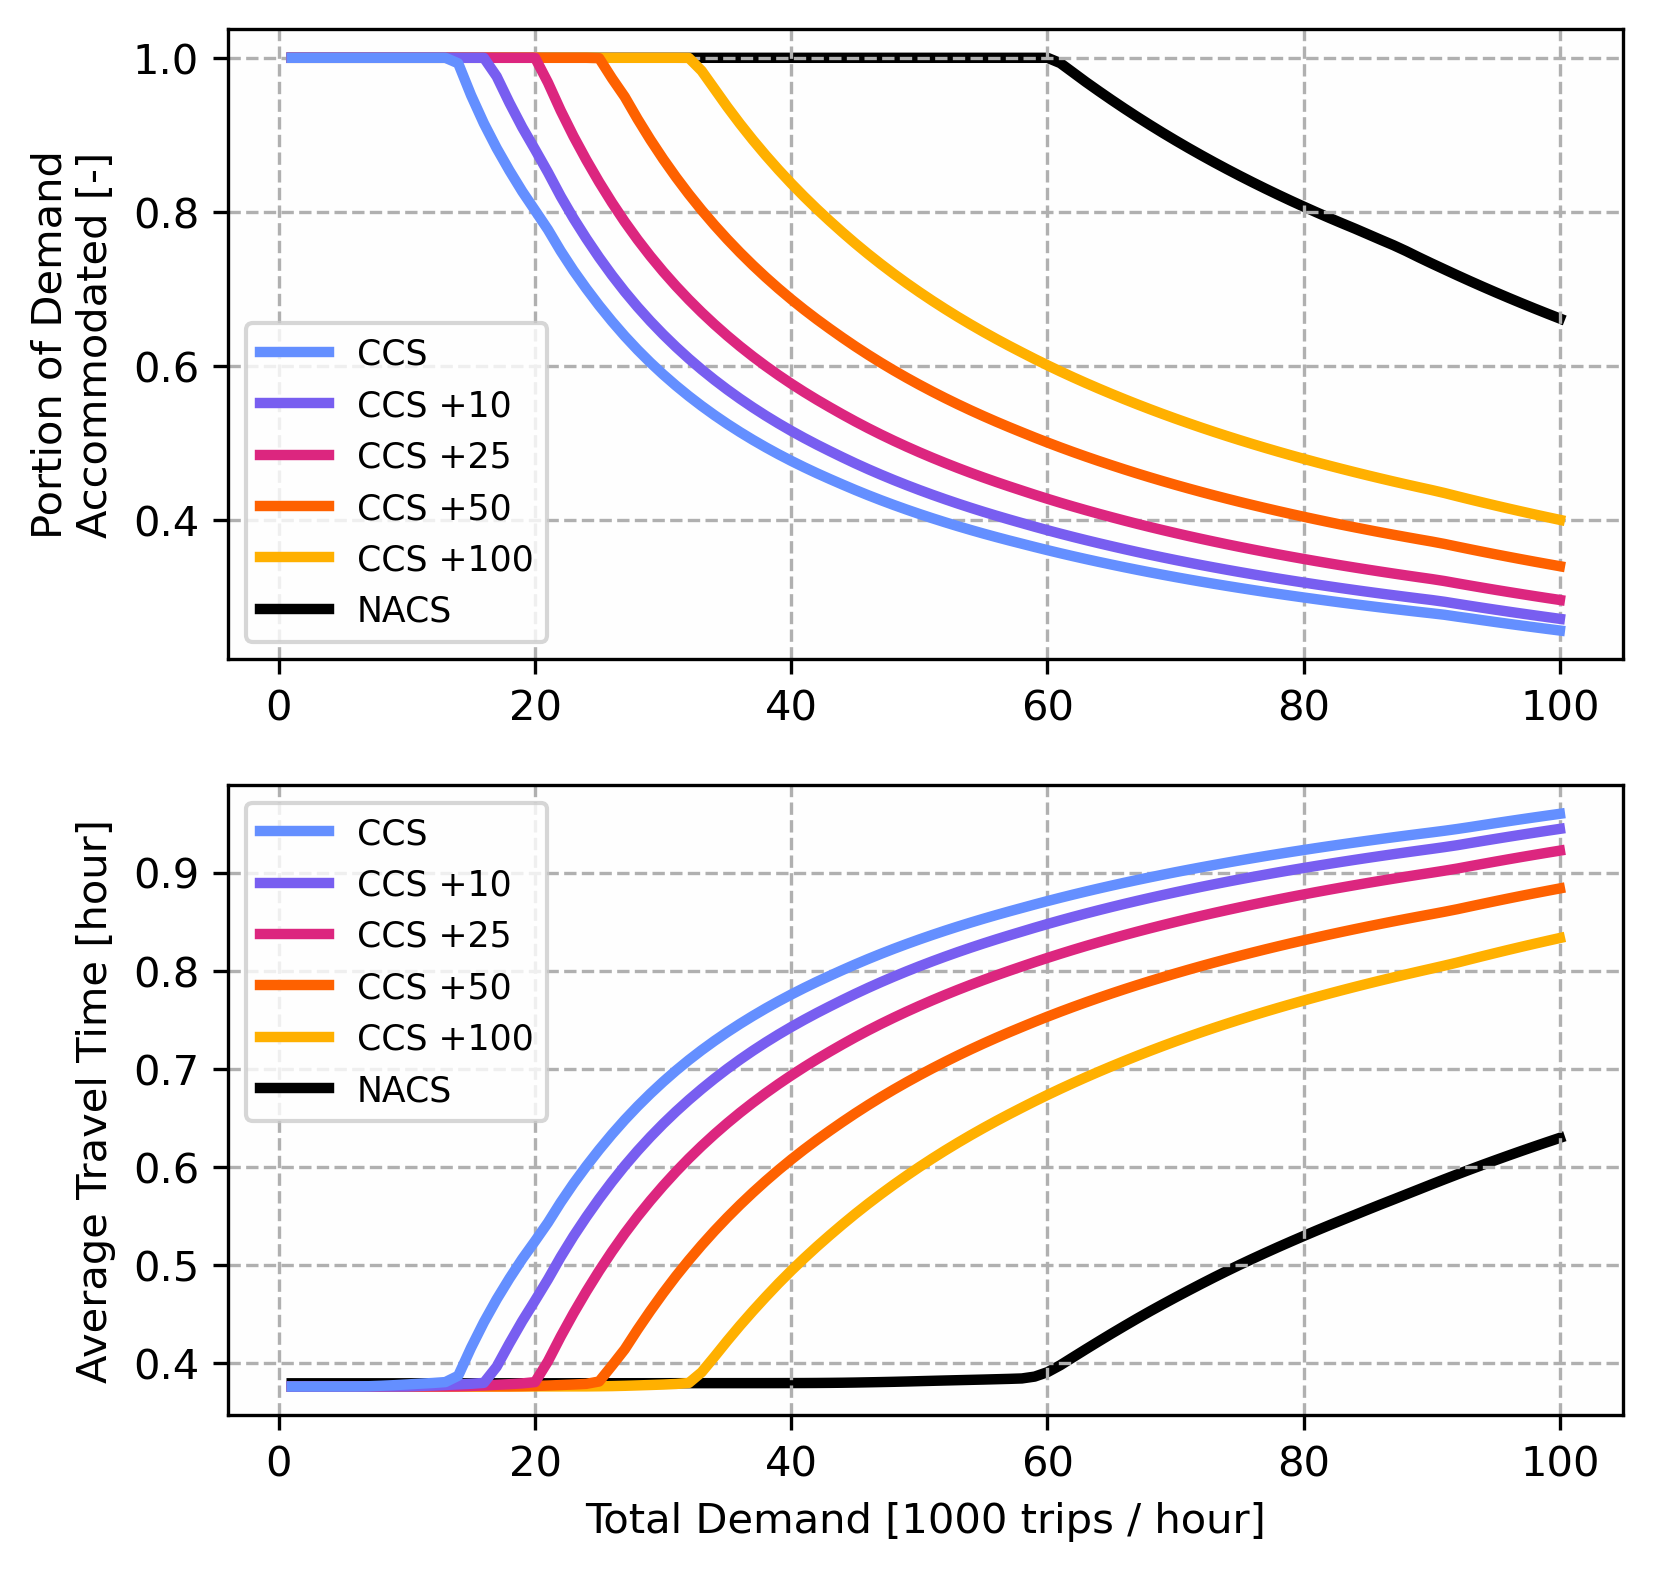
\includegraphics[width = \linewidth]{./figures/augmented_esn_performance.png}
	\caption{Performance of NACS, CCS, and augmented CCS \glspl{esn} with increasing demand.}
	\label{fig:augmented_esn_performance}
\end{figure}

Per the optimization results, substantial improvements in \gls{esn} performance can be attained by the strategic addition of a small number of chargers if they are allocated to form large stations in high traffic locations. The large stations added along Interstate 5 offer two benefits. The first is the already discussed benefit of increased station efficiency. The second benefit is increasing the number of trips along Interstate 5 as opposed to CA-99. Interstate 5 is a more direct route and has a higher speed limit. Vehicles traveling across the 5-99 corridor on Interstate save substantial driving time. As currently configures, the CCS \gls{esn} has more capacity along CA-99 and, thus, as the number of vehicles increases a higher portion are sent along this route. With the addition of several large stations along Interstate 5, much of this traffic can take Interstate 5 instead.




